\documentclass[12pt,a4paper,oneside]{report}
\usepackage[utf8]{inputenc}
\usepackage[T1]{fontenc}
\usepackage[french]{babel}
\usepackage{geometry}
\geometry{top=2.5cm, bottom=2.5cm, left=2.5cm, right=2.5cm}
\usepackage{graphicx}
\usepackage{amsmath}
\usepackage{amssymb}
\usepackage{booktabs}
\usepackage{hyperref}
\usepackage{listings}
\usepackage{xcolor}
\usepackage{caption}
\usepackage{float}

% Configuration des blocs de code
\definecolor{codegreen}{rgb}{0,0.6,0}
\definecolor{codegray}{rgb}{0.5,0.5,0.5}
\definecolor{codepurple}{rgb}{0.58,0,0.82}
\definecolor{backcolour}{rgb}{0.95,0.95,0.92}

\lstdefinestyle{mystyle}{
    backgroundcolor=\color{backcolour},   
    commentstyle=\color{codegreen},
    keywordstyle=\color{magenta},
    numberstyle=\tiny\color{codegray},
    stringstyle=\color{codepurple},
    basicstyle=\ttfamily\footnotesize,
    breakatwhitespace=false,         
    breaklines=true,                 
    captionpos=b,                    
    keepspaces=true,                 
    numbers=left,                    
    numbersep=5pt,                  
    showspaces=false,                
    showstringspaces=false,
    showtabs=false,                  
    tabsize=2
}
\lstset{style=mystyle}

\hypersetup{
    colorlinks=true,
    linkcolor=blue,
    filecolor=magenta,      
    urlcolor=cyan,
    pdftitle={Rapport de Projet - Deep Learning PyTorch},
    pdfpagemode=FullScreen,
}

\begin{document}

% ---------------------------------------------------------
% PAGE DE GARDE
% ---------------------------------------------------------
\begin{titlepage}
    \begin{center}
        \large\textbf{ÉCOLE MAROCAINE DES SCIENCES DE L'INGÉNIEUR} \\
        \large\textbf{EMSI} \\
        \vspace{1cm}
        \textbf{[LOGO EMSI]} \\ % Remplacer par \includegraphics{logo_emsi} lorsque le fichier sera disponible
        \hfill
        \vspace{1cm}
        
        \large\textbf{RAPPORT DE PROJET} \\
        \large\textbf{MODULE : DEEP LEARNING} \\
        \vspace{1.5cm}
        
        \hrule
        \vspace{0.4cm}
        {\huge \bfseries Implémentation et Analyse de Modèles de Deep Learning avec PyTorch} \\
        \vspace{0.2cm}
        {\large Classification d'Images (Fashion-MNIST) et Analyse de Sentiments (IMDb)}
        \vspace{0.4cm}
        \hrule
        
        \vspace{2.5cm}
        
        \begin{minipage}{0.45\textwidth}
            \begin{flushleft} \large
                \emph{Rédigé par :}\\
                \textbf{[Nom de l'Étudiant]} \\
                Élève Ingénieur
            \end{flushleft}
        \end{minipage}
        \hfill
        \begin{minipage}{0.45\textwidth}
            \begin{flushright} \large
                \emph{Encadré par :}\\
                \textbf{[Nom du Professeur]} \\
                Enseignant - EMSI
            \end{flushright}
        \end{minipage}
        
        \vfill
        \large Année Universitaire : 2025 -- 2026
    \end{center}
\end{titlepage}

% ---------------------------------------------------------
% REMERCIEMENTS
% ---------------------------------------------------------
\chapter*{Remerciements}
\addcontentsline{toc}{chapter}{Remerciements}

Je tiens à exprimer ma profonde gratitude à mon professeur et encadrant pour son orientation, ses précieux conseils et son soutien tout au long de ce projet de Deep Learning.

Mes remerciements s'adressent également à l'administration et au corps enseignant de l'École Marocaine des Sciences de l'Ingénieur (EMSI) pour avoir mis à notre disposition les ressources pédagogiques nécessaires à la réussite de ce travail.

Enfin, je remercie toute personne ayant contribué de près ou de loin à l'élaboration de ce projet.

% ---------------------------------------------------------
% RÉSUMÉ
% ---------------------------------------------------------
\chapter*{Résumé}
\addcontentsline{toc}{chapter}{Résumé}

Ce projet présente la conception, l'implémentation et l'évaluation de deux architectures de réseaux de neurones profonds en utilisant le framework PyTorch. 

La première partie est dédiée à la vision par ordinateur, où un réseau de neurones convolutif (CNN), nommé \texttt{FashionCNN}, est développé pour classifier les articles de mode du jeu de données \textbf{Fashion-MNIST}. Ce modèle est composé de deux couches convolutives suivies de couches de Max Pooling, d'un Dropout et de couches denses. 

La seconde partie traite de l'analyse de sentiments dans le domaine du traitement du langage naturel (NLP). Un modèle d'embedding continu avec pooling moyen (\texttt{SentimentModel}) est entraîné sur le jeu de données **IMDb Movie Reviews** pour classer des critiques de films comme positives ou négatives.

Ce rapport détaille la méthodologie adoptée, le prétraitement des données, les architectures choisies, les expérimentations menées et une analyse rigoureuse des résultats obtenus, illustrée par les courbes de perte (loss) et les visualisations d'erreurs réelles issues de l'exécution du projet.

% ---------------------------------------------------------
% TABLE DES MATIÈRES
% ---------------------------------------------------------
\tableofcontents

% ---------------------------------------------------------
% INTRODUCTION
% ---------------------------------------------------------
\chapter{Introduction}

\section{Contexte}
Dans le domaine de l'intelligence artificielle, le Deep Learning a révolutionné la façon dont les machines traitent les données complexes comme les images et le texte. Ce projet s'inscrit dans le cadre de notre formation d'ingénieur à l'EMSI, visant à acquérir une maîtrise pratique du framework PyTorch, l'un des standards industriels et académiques pour la conception de réseaux de neurones.

\section{Objectifs du Projet}
Ce projet vise à résoudre deux problématiques représentatives de l'apprentissage profond :
\begin{enumerate}
    \item \textbf{La classification multiclasse d'images} : Identifier automatiquement le type de vêtement représenté sur une image en niveaux de gris (10 classes possibles).
    \item \textbf{La classification binaire de textes} : Analyser une critique de film textuelle afin de prédire si l'opinion émise est positive ou négative.
\end{enumerate}

Le projet privilégie une approche modulaire et structurée pour assurer la maintenabilité et la clarté du code source.

% ---------------------------------------------------------
% PRÉSENTATION DU PROBLÈME ET DATASETS
% ---------------------------------------------------------
\chapter{Présentation du Problème et Données}

\section{Classification d'Images (Fashion-MNIST)}
Le premier problème consiste à classifier des images de vêtements de $28 \times 28$ pixels. Contrairement au traditionnel dataset MNIST (chiffres manuscrits), Fashion-MNIST présente une complexité accrue en raison de la diversité des textures et des motifs des articles.

\subsection{Description du Dataset}
Fashion-MNIST contient 70 000 exemples au total :
\begin{itemize}
    \item \textbf{Jeu d'entraînement} : 60 000 images.
    \item \textbf{Jeu de test} : 10 000 images.
\end{itemize}
Chaque image est étiquetée parmi les 10 classes suivantes :
\begin{table}[H]
    \centering
    \caption{Classes du jeu de données Fashion-MNIST}
    \begin{tabular}{clcl}
        \toprule
        Index & Classe & Index & Classe \\
        \midrule
        0 & T-shirt & 5 & Sandale \\
        1 & Pantalon & 6 & Chemise \\
        2 & Pull & 7 & Sneaker \\
        3 & Robe & 8 & Sac \\
        4 & Manteau & 9 & Bottine \\
        \bottomrule
    \end{tabular}
    \label{tab:fashion_classes}
\end{table}

\section{Analyse de Sentiments (IMDb)}
Le deuxième problème est une tâche de classification de texte binaire. Il s'agit d'analyser le sentiment général d'une critique de film.

\subsection{Description du Dataset}
Le dataset IMDb Movie Reviews comporte 50 000 critiques de films hautement polarisées récupérées sur le site IMDb :
\begin{itemize}
    \item \textbf{Jeu d'entraînement} : 25 000 critiques.
    \item \textbf{Jeu de test} : 25 000 critiques.
\end{itemize}
Les deux classes sont équitablement réparties (50\% de critiques positives et 50\% de critiques négatives).

% ---------------------------------------------------------
% MÉTHODOLOGIE ET ARCHITECTURES
% ---------------------------------------------------------
\chapter{Méthodologie et Implémentation}

Le projet est structuré de manière modulaire afin d'isoler les modèles, le chargement des données et les routines d'entraînement.

\section{Prétraitement des Données}

\subsection{Données Fashion-MNIST}
Les images brutes subissent une chaîne de transformations :
\begin{itemize}
    \item Conversion en tenseur PyTorch via \texttt{transforms.ToTensor()}, normalisant les intensités de pixels de $[0, 255]$ à $[0.0, 1.0]$.
    \item Normalisation avec une moyenne de $0.5$ et un écart-type de $0.5$ via \texttt{transforms.Normalize((0.5,), (0.5,))}, recentrant les valeurs autour de $[-1.0, 1.0]$.
\end{itemize}

\subsection{Données IMDb}
Pour les textes IMDb, un prétraitement spécifique est codé dans \texttt{SentimentDataset} :
\begin{enumerate}
    \item Le texte est converti en minuscules et découpé en mots simples (tokenisation par espace).
    \item Une troncature à une longueur fixe $L_{max} = 50$ mots est appliquée.
    \item Les mots sont convertis en indices entiers grâce à un vocabulaire pré-construit des 10 000 mots les plus fréquents. Les mots absents reçoivent l'index $1$ (\texttt{<UNK>}).
    \item Un rembourrage (\textit{padding}) à base de zéros (\texttt{<PAD>}) est ajouté pour atteindre la longueur fixe de 50.
\end{enumerate}

\section{Architectures des Modèles}

\subsection{Modèle de Vision : \texttt{FashionCNN}}
Défini dans \texttt{models/model.py}, le modèle utilise l'architecture suivante :
\begin{itemize}
    \item \textbf{Conv2D 1} : Canal d'entrée = 1, Canaux de sortie = 32, Noyau = $3\times3$, Padding = 1.
    \item \textbf{ReLU} suivie de \textbf{MaxPool2D} ($2\times2$, stride = 2) $\to$ Taille de sortie : $32 \times 14 \times 14$.
    \item \textbf{Conv2D 2} : Canaux d'entrée = 32, Canaux de sortie = 64, Noyau = $3\times3$, Padding = 1.
    \item \textbf{ReLU} suivie de \textbf{MaxPool2D} ($2\times2$, stride = 2) $\to$ Taille de sortie : $64 \times 7 \times 7$.
    \item \textbf{Flattening} : Transformation du tenseur $64 \times 7 \times 7$ en un vecteur unidimensionnel de taille 3136.
    \item \textbf{Linear 1} : Taille d'entrée = 3136, Taille de sortie = 128, suivie d'une fonction d'activation ReLU.
    \item \textbf{Dropout} : Taux de 25\% pour limiter le surapprentissage.
    \item \textbf{Linear 2 (Sortie)} : Taille d'entrée = 128, Taille de sortie = 10 (une pour chaque classe).
\end{itemize}

\subsection{Modèle NLP : \texttt{SentimentModel}}
Défini dans \texttt{models/sentiment_model.py}, le réseau est structuré ainsi :
\begin{itemize}
    \item \textbf{Embedding Layer} : Taille du vocabulaire $\times$ 64 dimensions. Traduit chaque mot en un vecteur continu. Le padding à l'index 0 est ignoré.
    \item \textbf{Global Average Pooling} : Calcule la moyenne des embeddings sur l'axe de la séquence de texte pour obtenir un vecteur unique représentatif du texte.
    \item \textbf{Linear Layer} : Taille d'entrée = 64, Taille de sortie = 1 (valeur brute pré-sigmoïdienne).
\end{itemize}

\section{Environnement de Développement et Outils}
\begin{itemize}
    \item \textbf{Langage} : Python.
    \item **Framework Principal** : PyTorch (gestion des tenseurs, rétropropagation, couches neuronales).
    \item \textbf{Visualisation} : Matplotlib (tracé des courbes de loss et visualisation d'images).
    \item \textbf{NLP} : Hugging Face \texttt{datasets} pour le téléchargement robuste de IMDb.
    \item \textbf{Métriques} : Scikit-learn (pour le calcul du rapport de classification).
\end{itemize}

% ---------------------------------------------------------
% EXPÉRIMENTATIONS ET RÉSULTATS
% ---------------------------------------------------------
\chapter{Expérimentations et Résultats}

\section{Entraînement des Modèles}
Les deux modèles ont été entraînés sur 5 époques avec l'optimiseur \textbf{Adam} (taux d'apprentissage $\eta = 0.001$).
*   Pour \texttt{FashionCNN}, la fonction de perte utilisée est \texttt{CrossEntropyLoss}.
*   Pour \texttt{SentimentModel}, la fonction de perte est \texttt{BCEWithLogitsLoss}.

\section{Résultats Obtenus}

\subsection{Classification Fashion-MNIST}
L'exécution de la boucle d'entraînement affiche la diminution progressive de la perte par époque.
\begin{table}[H]
    \centering
    \caption{Pertes enregistrées pendant l'entraînement de FashionCNN}
    \begin{tabular}{cc}
        \toprule
        Époque & Somme des pertes (Loss cumulée) \\
        \midrule
        1 & 392.2036 \\
        2 & 260.4079 \\
        3 & 220.8927 \\
        4 & 195.9680 \\
        5 & 175.7602 \\
        \bottomrule
    \end{tabular}
    \label{tab:loss_fashion}
\end{table}

À l'issue de l'entraînement, l'évaluation du modèle sur le jeu de test affiche les performances suivantes :
\begin{itemize}
    \item \textbf{Précision (Accuracy)} : 91.13\%
\end{itemize}

\subsection{Analyse de Sentiments IMDb}
Le tableau suivant résume la diminution de la loss du modèle d'embedding sur 5 époques.
\begin{table}[H]
    \centering
    \caption{Pertes enregistrées pendant l'entraînement de SentimentModel}
    \begin{tabular}{cc}
        \toprule
        Époque & Somme des pertes (Loss cumulée) \\
        \midrule
        1 & 265.3129 \\
        2 & 232.0837 \\
        3 & 207.9863 \\
        4 & 191.1311 \\
        5 & 178.6923 \\
        \bottomrule
    \end{tabular}
    \label{tab:loss_sentiment}
\end{table}

L'évaluation finale sur le jeu de test fournit le rapport de classification suivant :
\begin{table}[H]
    \centering
    \caption{Rapport de performance - Sentiment IMDb}
    \begin{tabular}{lcccc}
        \toprule
        Classe & Précision & Rappel & F1-Score & Support \\
        \midrule
        Négatif & 0.77 & 0.79 & 0.78 & 12500 \\
        Positif & 0.78 & 0.77 & 0.77 & 12500 \\
        \midrule
        \textbf{Global (Accuracy)} & & & \textbf{0.78} & 25000 \\
        \bottomrule
    \end{tabular}
    \label{tab:report_sentiment}
\end{table}

% ---------------------------------------------------------
% ANALYSE ET ENREGISTREMENTS GRAPHIQUES
% ---------------------------------------------------------
\chapter{Analyse et Discussion}

\section{Courbes de Perte (Loss)}
Les figures générées lors de l'exécution montrent la convergence des modèles.

\begin{figure}[H]
    \centering
    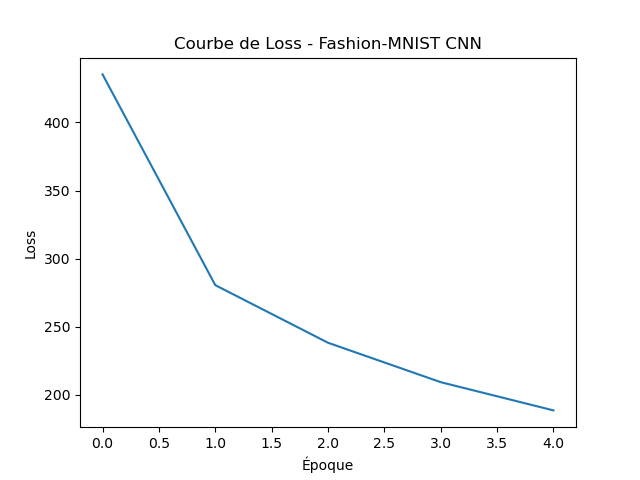
\includegraphics[width=0.7\textwidth]{loss_curve_fashion}
    \caption{Courbe de perte (Loss) de FashionCNN}
    \label{fig:loss_fashion}
\end{figure}

La courbe décroît régulièrement, indiquant un apprentissage stable sans divergence majeure sur les 5 époques programmées.

\begin{figure}[H]
    \centering
    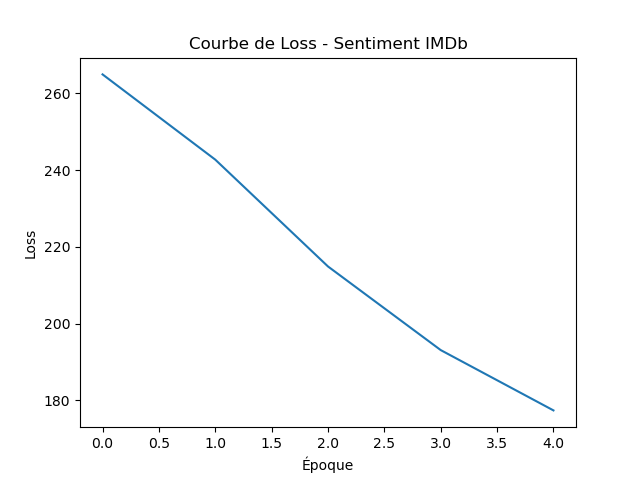
\includegraphics[width=0.7\textwidth]{loss_sentiment}
    \caption{Courbe de perte (Loss) de SentimentModel sur IMDb}
    \label{fig:loss_sentiment}
\end{figure}

\section{Visualisation et Analyse des Erreurs (FashionCNN)}
Le script extrait les prédictions erronées sur l'ensemble de test et les enregistre dans \texttt{erreurs_fashion.png}.
\begin{figure}[H]
    \centering
    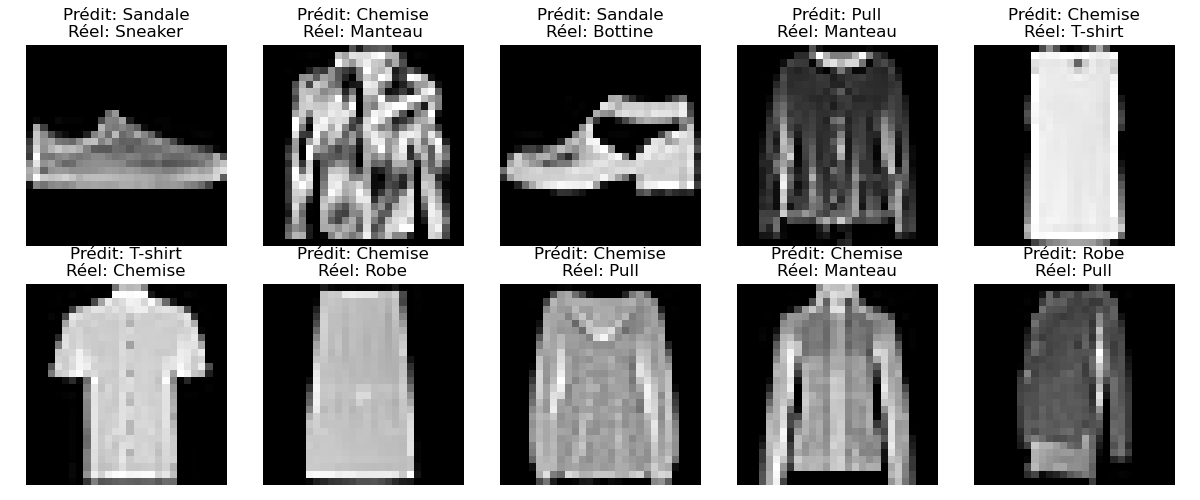
\includegraphics[width=0.85\textwidth]{erreurs_fashion}
    \caption{Exemple de 10 prédictions incorrectes de FashionCNN}
    \label{fig:erreurs_fashion}
\end{figure}

L'analyse de ces images montre que la plupart des erreurs proviennent de confusions logiques entre des catégories visuellement très similaires :
\begin{itemize}
    \item Confusion récurrente entre les classes **Pull** (Pullover), **Manteau** (Coat) et **Chemise** (Shirt).
    \item Confusion entre les chaussures : **Sandale**, **Sneaker** et **Bottine**.
\end{itemize}
Ces erreurs sont partagées même par des observateurs humains sur des images basse résolution en niveaux de gris.

\section{Limites du Modèle d'Analyse de Sentiment}
L'accuracy globale plafonne à 78\%. Cette performance modeste s'explique par les limitations suivantes :
\begin{enumerate}
    \item **Perte d'informations temporelles** : Le modèle fait la moyenne des embeddings. Deux phrases avec les mêmes mots dans un ordre différent auront la même signature d'embedding.
    \item **Taille fixe trop courte** : Fixer la longueur des textes à 50 mots tronque la majorité des avis IMDb, perdant ainsi le contexte de fin de critique.
    \item **Tokenisation rudimentaire** : L'absence de nettoyage de la ponctuation fragmente inutilement le dictionnaire (ex: "super!" et "super" comptent pour deux mots distincts).
\end{enumerate}

% ---------------------------------------------------------
% DIFFICULTÉS ET CONCLUSION
% ---------------------------------------------------------
\chapter{Difficultés Rencontrées et Conclusion}

\section{Difficultés Rencontrées}
\begin{itemize}
    \item \textbf{Problème de bibliothèque doublée (KMP Duplicate Lib)} : Une erreur liée à l'environnement d'exécution OpenMP sous Windows a nécessité l'utilisation de la variable d'environnement \texttt{os.environ["KMP\_DUPLICATE\_LIB\_OK"] = "TRUE"}.
    \item \textbf{Duplication de code} : Les versions obsolètes des codes d'entraînement et d'évaluation dans les fichiers de départ rendaient le débogage complexe (absence de \texttt{model.eval()} et de \texttt{model.train()} dans certaines branches).
    \item \textbf{Limitations matérielles} : L'exécution du jeu de données IMDb sur CPU ralentit grandement la vitesse d'apprentissage de l'embedding.
\end{itemize}

\section{Conclusion et Perspectives}
Ce projet a permis de mettre en œuvre deux pipelines complets de Deep Learning avec PyTorch. Le modèle CNN a montré une très bonne efficacité pour le traitement d'images (91.13\% d'accuracy), tandis que le modèle d'embedding sur le texte a posé les bases de la classification en NLP.

Pour de futures itérations, nous envisageons :
\begin{itemize}
    \item L'intégration d'un réseau récurrent (LSTM/GRU) ou d'un CNN 1D pour l'analyse de texte.
    \item La mise en œuvre d'un script de détection automatique pour exploiter l'accélération matérielle GPU (CUDA).
\end{itemize}

% ---------------------------------------------------------
% BIBLIOGRAPHIE
% ---------------------------------------------------------
\begin{thebibliography}{9}
\bibitem{pytorch}
  Adam Paszke, Sam Gross, Francisco Massa, et al.
  \emph{PyTorch: An Imperative Style, High-Performance Deep Learning Library}.
  Advances in Neural Information Processing Systems 32 (NeurIPS 2019).

\bibitem{fashionmnist}
  Han Xiao, Kashif Rasul, Roland Vollgraf.
  \emph{Fashion-MNIST: a Novel Image Dataset for Benchmarking Machine Learning Algorithms}.
  arXiv:1708.07747, 2017.

\bibitem{imdb}
  Andrew L. Maas, Raymond E. Daly, Peter T. Pham, Dan Huang, Andrew Y. Ng, and Christopher Potts.
  \emph{Learning Word Vectors for Sentiment Analysis}.
  Association for Computational Linguistics (ACL), 2011.
\end{thebibliography}

\end{document}
